\documentclass{llncs}
\usepackage{graphicx}
\usepackage{wrapfig}
\usepackage{algorithm2e}
\usepackage{fancyvrb}

\newcommand{\hide}[1]{}

\title{BULL: a Library for Learning Algorithms of Boolean Functions }
\author{Yu-Fang Chen \and Bow-Yaw Wang}

\institute{Academia Sinica, Taiwan}

\pagestyle{plain}
\sloppy

\begin{document}
\maketitle

\begin{abstract}%0.3
\hide{
Learning algorithms for Boolean functions have recently been applied
in various applications of formal verification such as automated
compositional reasoning and finding loop invariants.
}
We present the tool BULL (Boolean fUnction Learning Library), the
first publicly available implementation of learning algorithms for
Boolean functions.
The tool is implemented in C with interfaces to C++, JAVA and OCAML.
Experimental results show significant advantages of Boolean function
learning algorithms over all variants of the $L^*$ learning
algorithm for regular languages.\\
\hide{
For instance, our implementation is
able to infer a 12-bit counter machine model in less than 2 minutes,
while the best algorithm implemented in libalf fails to find it within
an hour.\\
}

\centering
Web-site: \verb"http://bull.iis.sinica.edu.tw/"

\end{abstract}
\vspace{-1.2cm}
\section{Introduction} %1p
% what is it

BULL is the first publicly available implementation of learning
algorithms for Boolean functions. Three learning algorithms are
implemented in the library. The classical \textmd{CDNF} algorithm
infers Boolean functions over a fixed number of variables. The
incremental \textmd{CDNF+} and \textmd{CDNF++} algorithms infers
Boolean functions over an indefinitely number of variables. The
library is implemented in C with C++, JAVA and OCAML interfaces.
Sample codes of C, C++, JAVA, and OCAML are distributed with the
library. Users can adopt BULL by modifying them.

\vspace{-4mm}
\subsubsection*{What is it?} Learning algorithms for Boolean functions can be viewed as an
efficient procedure to generate a \emph{target} Boolean function
only known to a teacher. This type of learning algorithms assume
a teacher who can answer queries about the target Boolean
function. The learning algorithms acquire information from the answers
to queries and organize them in a systematic way. In the worst case,
learning algorithms will infer a target Boolean function within
a polynomial number of queries in the CNF and DNF formula sizes of the
target function.

%motivation
\vspace{-4mm}
\subsubsection*{Learning in formal verification.} Since the work in~\cite{MP:1995:OLIRS},
algorithmic learning has been applied to
formal verification techniques such as
specification synthesis~\cite{MP:1995:OLIRS}, automated compositional
verification~\cite{CGP:2003:LACV}, and regular model
checking~\cite{HV:05}. Most applications are based on the
$L^*$ automata learning algorithm for regular languages.
%To be more specific, the most used algorithm is Angluin's
%L*~\cite{a-lrsqc-87} or its variants such as Rivest and Schapire's
%algorithm~\cite{RS:1993:IFAUHS} and the tree-based algorithm of
%Kearns and Vazirani~\cite{KV:1994:ICLT}.
The learning algorithm enumerates states
explicitly, hence its applications are
inherently explicit~\cite{CGP:2003:LACV}, or use explicit automata
as implicit representations of state spaces~\cite{HV:05}.
\vspace{-4mm}
\subsubsection*{Why use Boolean learning.} Implicit algorithms (e.g., SAT-based model checking) can greatly improve the capacity of various
verification techniques. Similar improvements have also been reported
in applications of the \textmd{CDNF} learning algorithm for Boolean
functions. In~\cite{CCFTTW:10:AAGRIL}, the learning algorithm is
adopted to infer implicit contextual assumptions in automated
compositional reasoning. It is shown that learning implicitly
can tackle certain hard problems unattainable by traditional
explicit algorithms. The \textmd{CDNF} algorithm is also applied to
loop invariant generation. The learning-based framework can be
much more efficient than conventional static analysis
algorithms~\cite{JKWY:10:DIPL}.

For learning algorithms for regular languages, there are
mature and publicly available tools (such as libalf~\cite{libalf} and
learnlib~\cite{learnlib}). Implementations of learning algorithms for
Boolean functions however are still missing. Since it would take a
considerable amount
of time to understand and implement learning algorithms for Boolean
functions, lack of publicly available tools could be an obstacle to
develop related techniques in the research community. In order to
lower the barrier to entry, we decide to develop the BULL library.

\vspace{-4mm}
\subsubsection*{The Position of the Paper}
The Boolean learning project starts in 2009 and since
then we tested different variants of the algorithms and data
structures. Several of them indeed dramatically improved the
performance, e.g., non-membership queries are introduced
partly for performance reasons. 
However, since boolean learning is a new technique to most people in
the community. We decided to spend
the pages for a general introduction instead of technical details. 

\vspace{-5mm}
\section{The BULL Library}%0.5page

\vspace{-5mm}
\begin{wrapfigure}{l}{0.5\linewidth}
\vspace{-10mm}
\begin{center}
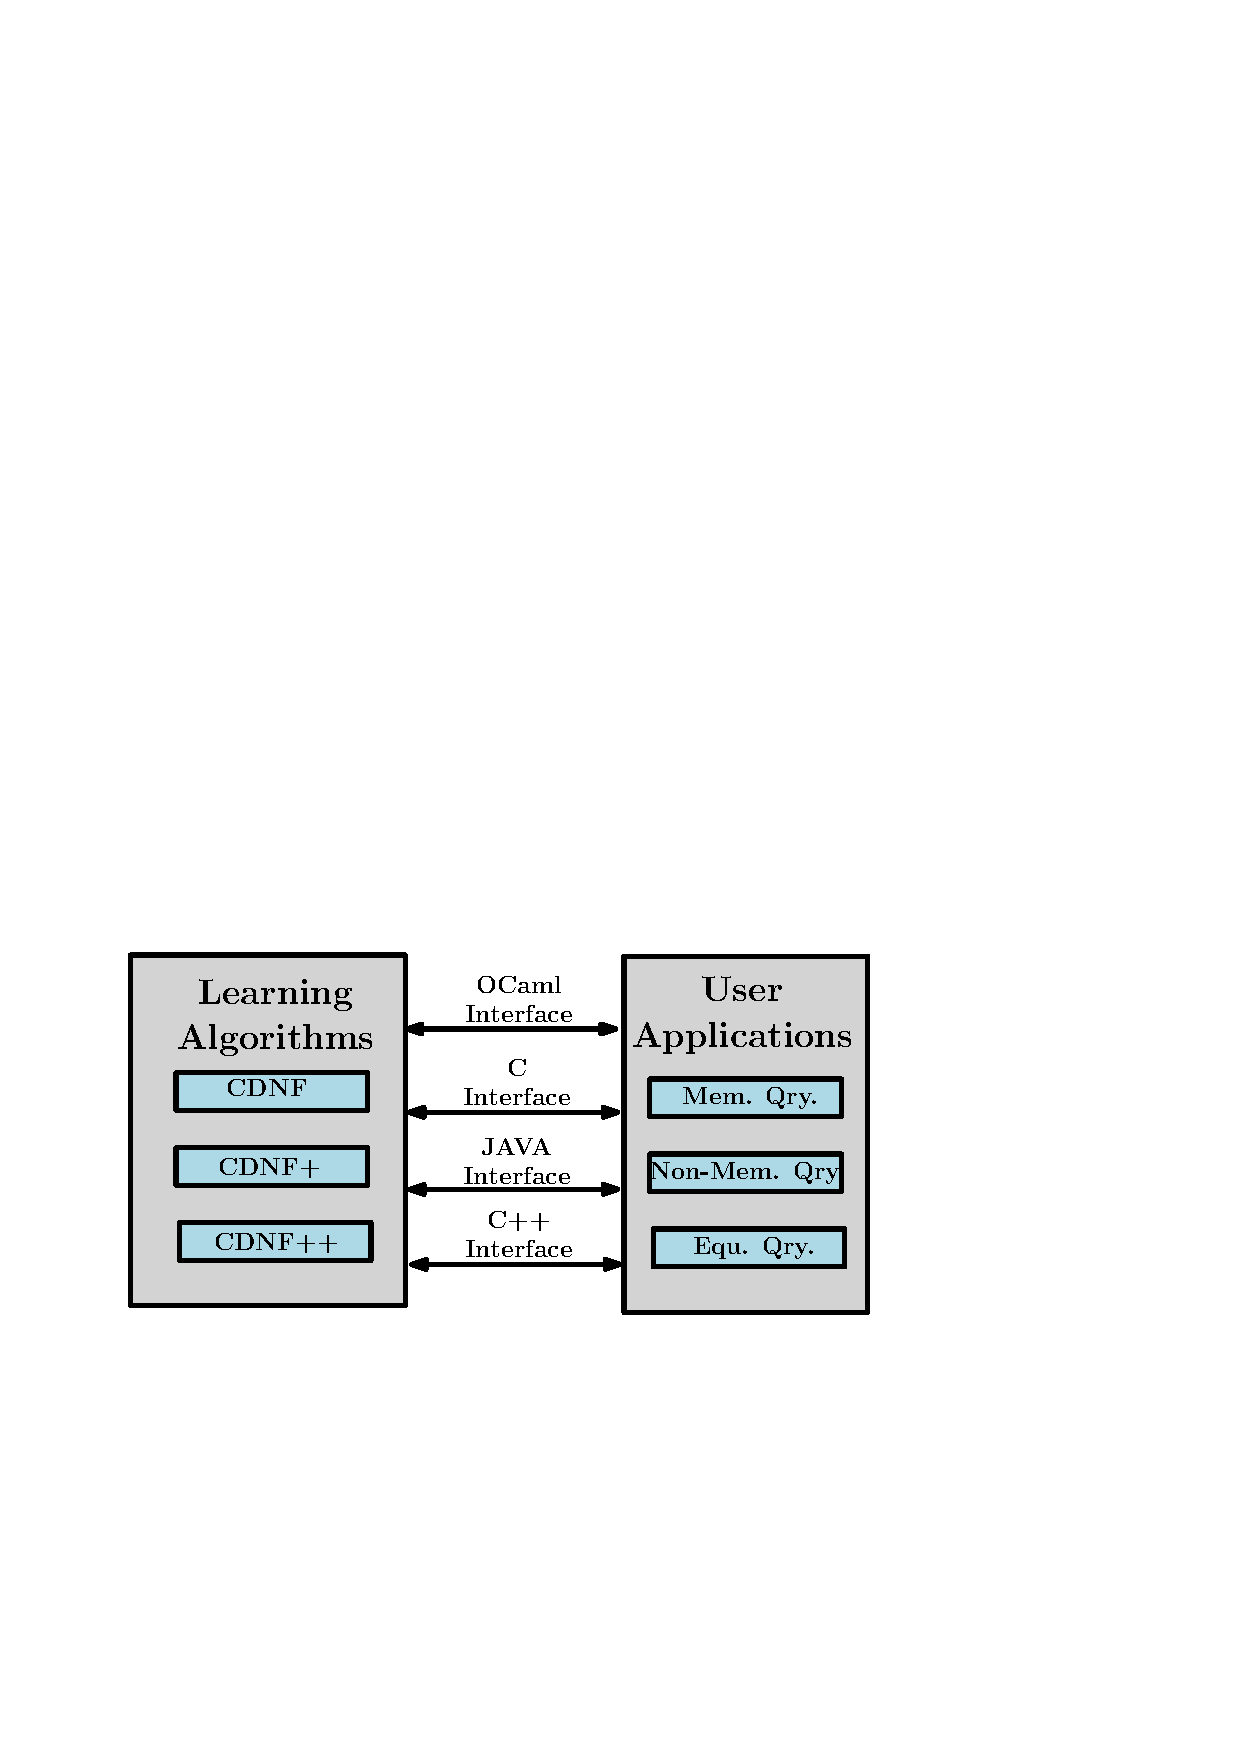
\includegraphics[scale=0.43]{figures/arch}
\vspace{-7mm}
\caption{System Architecture}
\label{fig:arch}
\end{center}
\vspace{-10mm}
\end{wrapfigure}

Figure~\ref{fig:arch} shows the architecture of BULL. The core library
contains three learning algorithms implemented in C. They are
the \textmd{CDNF}~\cite{B:95:ELBF}, \textmd{CDNF+}~\cite{CW12}, and
\textmd{CDNF++}~\cite{CW12} algorithms. The \textmd{CDNF} algorithm
assumes that the number of variables in the target Boolean function is
known. The \textmd{CDNF+} and \textmd{CDNF++} algorithms do not have
this assumption.
\hide{
For applications such as loop invariant
generation or function summaries, the number of variables in the
target Boolean function \emph{is unknown}. The latter two algorithms derived
from the CDNF algorithm are most suitable for such scenarios.
The outputs of these algorithms are Boolean formulae
the form of
CDNF (conjunction of formulae in disjunction normal form).
}
In addition to the learning algorithms, we also provide C++, JAVA (via JNI), 
and OCaml interfaces.

\vspace{-0.5cm}
\subsection{How to Use the Package}
In order to adopt the learning algorithms in BULL, users have to play
the teacher and answer queries posed by the algorithms. For the sake
of presentation, let us assume that $f(x, y, z) = (x \wedge \neg y) \vee (x
\wedge z)$ is the target Boolean function over variables $x, y,$ and
$z$. Consider the following sample queries from the learning algorithms:
\begin{enumerate}
\item A \emph{membership} query on a partial assignment $\{ (x,
  \mathit{false}) \}$. On a membership query, the teacher checks if
  the target is satisfiable under the given assignment. Here the teacher answers $\mathit{no}$ since $f (\mathit{false}, y, z)$ is
  not satisfiable.
\item A \emph{non-membership} query on a parital assignment $\{ (y,
  \mathit{true}) \}$. On a non-membership query, the teacher checks if
  the negation of the target is satisfiable under the
  assignment. For this example, the teacher answers $\mathit{yes}$.
\item An \emph{equivalence} query on a conjecture $f'(x,y,z)$. On an
  equivalence query, the teacher answer $\mathit{yes}$ if the given
  formula is equivalent to the target. Otherwise, she returns an
  assignment as a counterexample. For this example, the teacher may
  return the assignment $\{ (x, \mathit{true}), (y, \mathit{true}),
  (z, \mathit{false}) \}$ since $f' (\mathit{true}, \mathit{true},
  \mathit{false}) \neq f (\mathit{true}, \mathit{true},
  \mathit{false})$.
\end{enumerate}

Different learning algorithms pose different types of
queries. Table~\ref{tab:algimp} shows the differences among the
three learning algorithms in BULL.
\begin{table}[htdp]
\vspace{-0.4cm}
%\label{tab:algimp}
\begin{center}
\begin{tabular}{|c|c|c|c|c|}
\hline
&Num. of Vars. & Mem. Qry, & Non-Mem. Qry. & Equ. Qry. \\
\hline
CDNF& known& $\surd$ & & $\surd$\\
CDNF+& unknown& $\surd$ & & $\surd$\\
CDNF++& unknown& $\surd$ &$\surd$& $\surd$\\
\hline
\end{tabular}
\end{center}
\caption{Features of Algorithms}
\label{tab:algimp}
\end{table}%
\vspace{-1cm}
The \textmd{CDNF} algorithm assumes the number of variables in the
target Boolean function is known. The \textmd{CDNF+} algorithm does
not know the number of variables. Both algorithms only pose
membership and equivalence queries. The \textmd{CDNF++} algorithm does
not presume the number of variables is known. It however pose
membership, non-memberhip, and equivalence queries.

BULL defines the interfaces to the three types of queries. If all
queries can be answered automatically, users can implement a
mechanical teacher to answer queries through the interface. Learning
algorithms in BULL will invoke the mechanical teacher and infer
unknown target functions automatically.
We refer interested users to the appendix or our web-site for a detailed demonstration of 
how to implement the above query functions and connect them to BULL.

\hide{
(1) BULL may pose membership (co-membership) queries in order to obtain information about the target function. The user has to provide information about the target function by replying these queries with yes-or-no answers. To be more specific, for a \emph{membership query} on an (partial) assignment $v=\{(x, \mathit{false})\}$, the user should answer $\mathit{no}$ because the formula $f'$, obtained by replacing all occurrences of $x$ in the target function $f$ with $\mathit{false}$, has no satisfying assignment. On the other hand, for a \emph{co-membership query} on $v$, the user should answer $\mathit{yes}$, because the formula $\neg f'$ is satisfiable. (2) After collected a certain number of query results, BULL will pose an equivalence query on a conjecture Boolean function $c$ which it believes to be equivalent to the target function. The user should answer $\mathit{yes}$ when $c=f$. Otherwise, an assignment in the difference of the satisfying assignments of $c$ and $f$ should be returned to BULL to refine the next conjecture. For the latter case, BULL will loop back to steps (1),(2) and generates another conjecture. These loop iterations will be repeated and eventually converge to the target function.
}

\hide{
The above procedure can be done fully automatically. BULL provides interfaces of the above three types of queries. Users can define how to answer these queries by implementing functions follows these interfaces. The core of BULL will automatically invoke and interact with these implemented functions.
}

\hide{
After the needed interface functions are implemented, the users can choose/switch freely between the three learning algorithms implemented in BULL without any additional effort.

Below we list all the interface functions in BULL:
\begin{itemize}
\item \textbf{Mem($v$)}: Membership query on an assignment $v$ returns \emph{true} if $v$ is a \emph{satisfying assignment} of the target Boolean function. Otherwise returns \emph{false}.
\item \textbf{CoMem($v$)}: Co-Membership query on a assignment $v$ returns \emph{true} if $v$ is an \emph{unsatisfying assignment} of the target Boolean function. Otherwise returns \emph{false}.
\item \textbf{Equ($c$)}: Equivalence query on a conjecture Boolean function
  $c$ asks if $c$ is equivalent to the target Boolean function.
  In case that they are not equivalent, an assignment that
  differentiates the two is returned.
\end{itemize}

Notice that at the first glance, one might feel that the functionality of membership query and co-membership query are the same. However, the inputs of these two types of queries are not necessary

for membership and co-membership queries, free variables in the target Boolean function undefined in $v$ are existentially quantified.
Assume that the target function is $(x \wedge y)$ and an assignment $v=\{(x,\mathit{true})\}$.
Then a correct implementation of the interface functions should have the results \textbf{Mem($v$)}=\textbf{CoMem($v$)}=\textit{true}.
}

\hide{
\subsection{Algorithms Implemented in BULL}
Here we describe more details of the algorithms implemented in BULL. All the three algorithms have the same object, learning boolean function from a teacher (the user), and interact with the teacher in the same manner described in the previous subsection. The main difference of the three algorithms are described in Table~\ref{tab:algimp}.


\begin{table}[htdp]
\caption{Algorithms implemented}
%\label{tab:algimp}
\begin{center}
\begin{tabular}{|c|c|c|c|c|}
\hline
&Num. of Vars. & Mem. Qry, & Co-Mem. Qry. & Equ. Qry. \\
\hline
CDNF& known& $\surd$ & & $\surd$\\
CDNF+& unknown& $\surd$ & & $\surd$\\
CDNF++& unknown& $\surd$ &$\surd$& $\surd$\\
\hline
\end{tabular}
\end{center}
\label{tab:algimp}
\end{table}%

As mentioned before, CDNF needs to know the number of variables in the target function.
This information is not always available before the target function is found (e.g, when the learning algorithm is used to infer loop invariants or function summaries). CDNF+ and CDNF++
are developed for the situation when the number of variables in the target function cannot be known in advance. Although the latter two algorithms have the same functionality, CDNF+
requires a simpler teacher answering only two types of queries (equivalence and membership)
while CDNF++ has a better performance.
}

\subsection{Users of BULL}
The BULL library targets the formal verification research
community. As far as we know, several people in the field are
interested in the applications of learning algorithms for Boolean
functions. The library has already been used by the verification group
\hide{of Marta Kwiatkowska}
in Oxford University (Learning-based Compositional Probabilistic Model
Checking), the software trustability and verification group in
Tsinghua University (Learning-Based Compositional Verification),
and the static analysis group in Seoul National University (Loop Invariant
Inference). Several other groups have also expressed their interests and
asked for the source code.

\subsection{Potential Applications} %(1 pages)
The \textmd{CDNF} algorithm has been applied to synthesize
contextual assumptions in assume-guarantee reasoning.
It has also been used to infer a loop invariant in program
verification. These applications share common characteristics.
First, computing contextual assumptions or loop invariants
without learning is possible but expensive. It is however easy to
verify if purported contextual assumptions or loop invariants
work. Moreover, contextual assumptions or loop invariants are by no
mean unique. It suffices to compute but one contextual assumption or
loop invariant in these applications. From our experience, we believe
that learning is most suitable for problems with the aforementioned
characteristics.

The appendix explains how to use the BULL
library to find loop invariants in details. We hope it may give some
insights to more applications of the library.


\section{Experimental Results} %(1page)
We have two sets of experiments. In the first one, we
compare Boolean and automata learning
algorithms. In the second one, we compare three algorithms implemented in BULL using random 3SAT formulae.

\subsection{Compare Boolean Learning and Automata Learning Algorithms}
Compositional verification and fix-point calculation are
the two main applications of algorithmic learning in formal
verification. Both automata and Boolean learning have been used to
solve these problems. Since both learning algorithms can be used for
the same problem, we think a comparison between them would be interesting.

We compare algorithms implemented in BULL with five
automata learning algorithms implemented in libalf~\cite{libalf}.
The natures of the two types of learning algorithms are quite different; the target of automata learning is ``a language'' while the target of Boolean learning is more often ``a structure'' (e.g, a transition function). It is in general hard to compare them. There exists automata with complicated structure, but simple language (e.g., an automaton accepts $\Sigma^*$ can have very complicated structure). This type of automata can be easily learned by automata learning algorithm, but can be extremely hard for Boolean learning.

Since the target application of BULL is verification, we decide to pick a classical example, $n$-bit counter, as the target for learning (Table~\ref{tab:autboolcmp}). To be more specific, we use Boolean learning algorithms to target the circuit of a counter and automata learning algorithms to target the state machine obtained by unfolding the circuit.
In Table~\ref{tab:autboolcmp2},
we show a different version where the $n$-bit counter model can
be non-deterministically reset to 0 from any state. We use a timeout
period of 1 hour. Each entry of the table is the execution time in
seconds (``TO'' denotes timeout). Each row is the result of an algorithm and each column is the
number of bits used in the counter.  From the tables, we can see Boolean learning algorithms significantly outperform the automata learning algorithms in this type of models. For example, all of them can infer a 12-bit counter machine model in less than 2 minutes,
while the best algorithm implemented in libalf fails to find it within an hour.


\begin{table}[h]
\begin{center}
\begin{tabular}{|c|c|c|c|c|c|c|c|c|c|c|c|}
\hline
  &2&3&4&5&6&7&8&9&10&11&12\\
\hline
\hline
CDNF& 0.02&0.02&0.05&0.11&0.35&1.03&2.29& 4.3& 9.8& 23.6 &66.2\\
CDNF+& 0.01&0.02&0.04&0.09&0.27&0.77& 1.5& 2.4& 5.7 &14.1 & 40.3\\
CDNF++& 0.01&0.02&0.04&0.09&0.25&0.77& 1.5& 2.4& 5.6 &13.8 & 39.8\\
Angluin's L*  & 0.01 & 0.03 & 0.51 & 73.02 & TO & TO & TO& TO& TO& TO& TO\\
Angluin's L* (column-based)  & 0.03 & 0.08 & 1.81 & 316.95 & TO & TO & TO & TO& TO& TO& TO\\
Rivest \& Schapire's  & 0.02 & 0.02 & 0.14 & 2.47 & 174.71 &TO & TO& TO& TO& TO& TO\\
NL*  & 0.02 & 0.02 & 0.17 & 4.45 & 215.84 &TO & TO& TO& TO& TO& TO\\
Kearns \& Vazirani's  & 0.01 & 0.02 & 0.04 & 0.28 & 2.47 &18.54 & 96.65&787.7 &  TO & TO & TO \\
\hline
\end{tabular}
\caption{Comparison of automata and Boolean function learning algorithm: using n-bit counter as the example}
\label{tab:autboolcmp}
\end{center}
\vspace{-1cm}
\end{table}

\begin{table}[h]
\begin{center}
\begin{tabular}{|c|c|c|c|c|c|c|c|c|c|c|c|}
\hline
  &2&3&4&5&6&7&8&9&10&11&12\\
\hline
\hline
CDNF& 0.00&0.02&0.07&0.24&0.75&2.83&12.13&  32.01& 112 &451&1374\\
CDNF+& 0.01&0.02&0.06&0.21&0.67&2.63&  12.1& 36.8 &144&637& 1671\\
CDNF++& 0.01&0.02&0.06&0.21&0.62&2.63&12.08&  36.88& 145 &582&1632\\
Angluin's L*  & 0.01 & 0.02 & 0.14 & 2.52 & 146.11 & TO & TO& TO& TO& TO& TO\\
Angluin's L* (column-based)  & 0.03 & 0.08 & 1.78 & 313 & TO & TO & TO & TO& TO& TO& TO\\
Rivest \& Schapire's  & 0.01 & 0.02 & 0.15 & 2.64 & 164.2 &TO & TO& TO& TO& TO& TO\\
NL*  & 0.01 & 0.07 & 2.14 & 363.8 &TO & TO& TO& TO& TO& TO& TO\\
Kearns \& Vazirani's  & 0.01 & 0.02 & 0.06 & 0.45 & 4.61 &33.52 & 181.5& 1486.6&TO   & TO &TO\\
\hline
\end{tabular}
\caption{Comparison of automata and Boolean function learning algorithm: using n-bit counter with non-deterministic reset as the example}
\label{tab:autboolcmp2}
\end{center}
\vspace{-1cm}
\end{table}



\subsection{Compare Boolean Learning Algorithms using 3SAT Formulae}
\begin{figure}[htdp]
\begin{center}
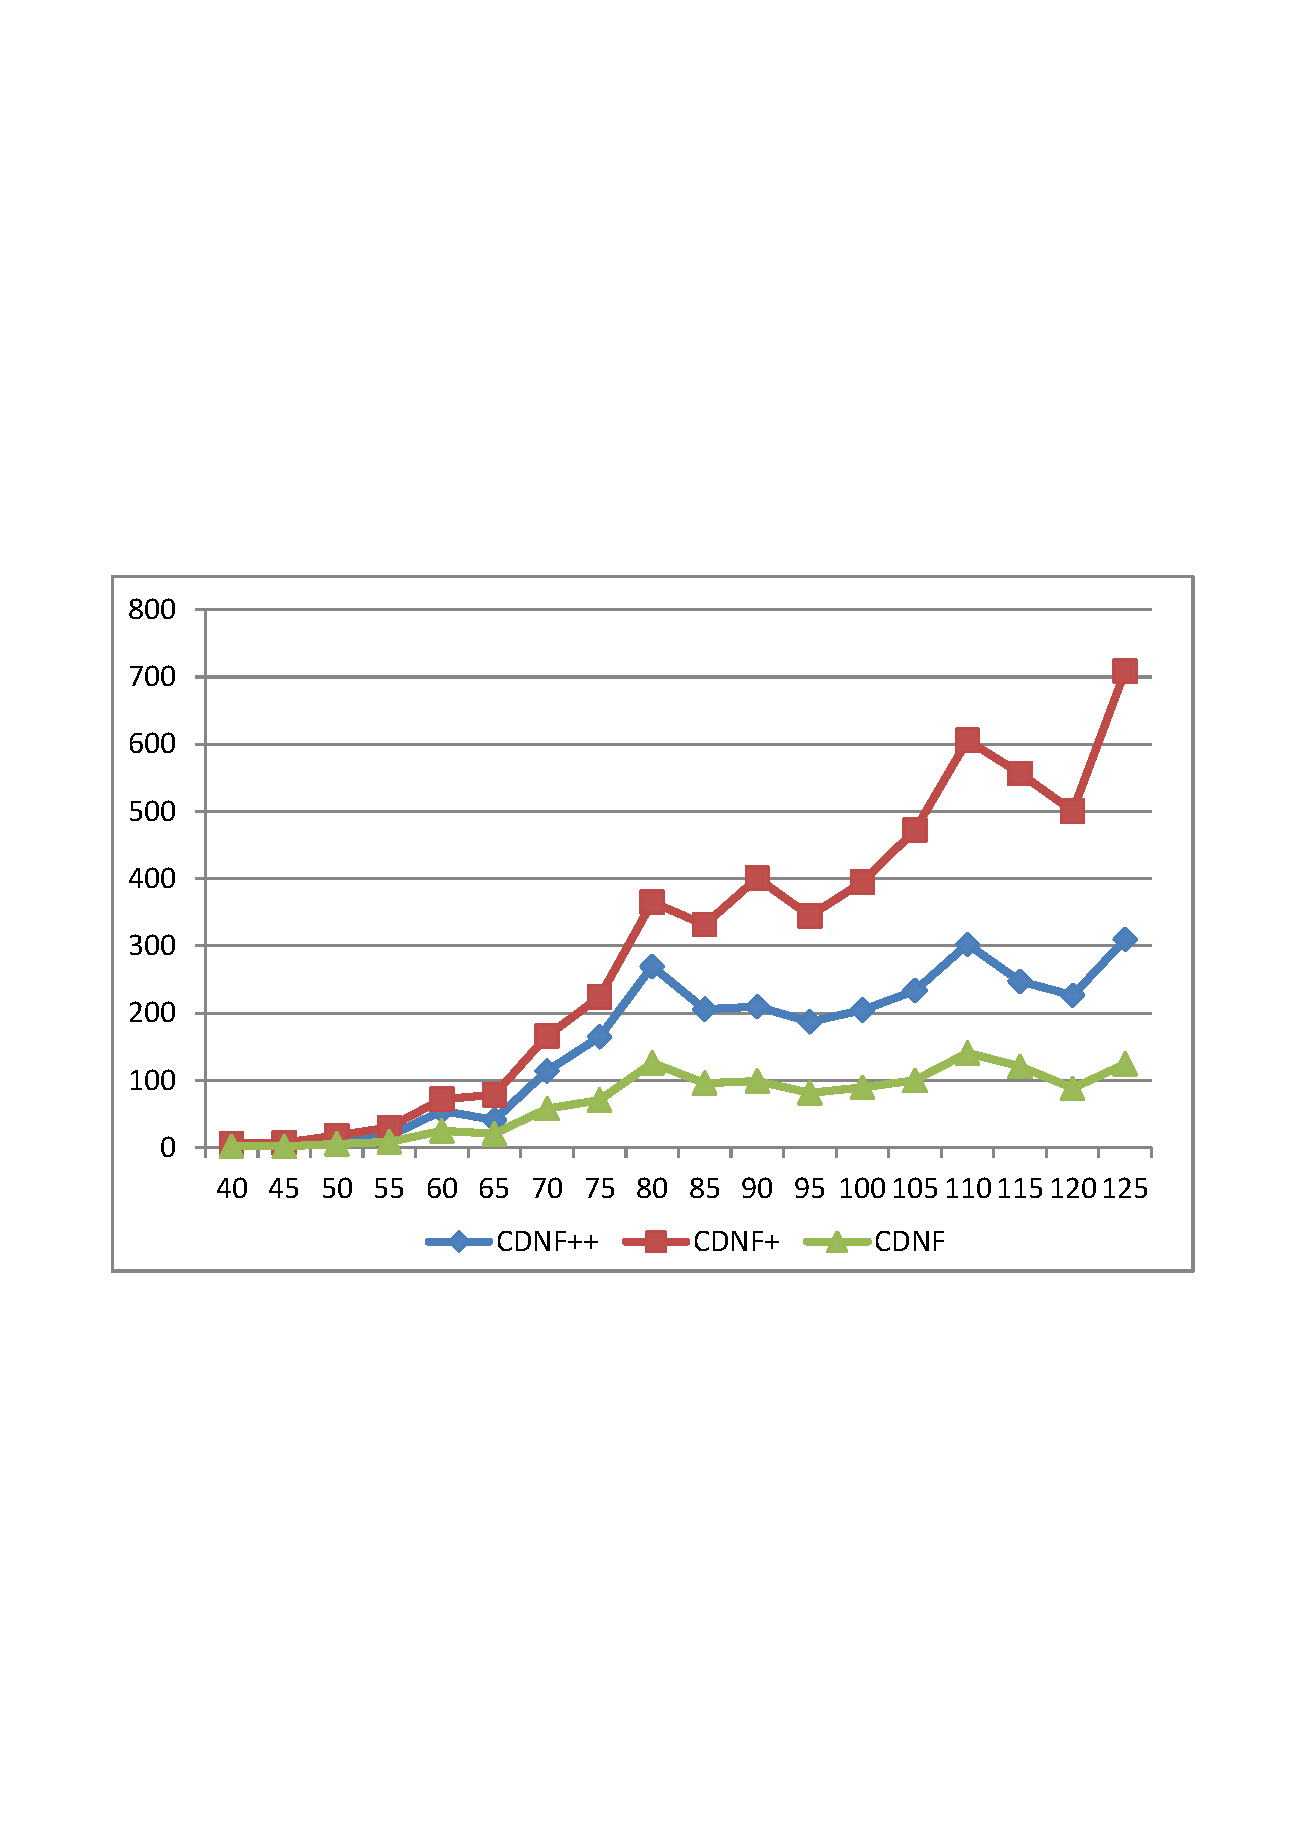
\includegraphics[scale=0.4]{figures/AVG}

\caption{Comparison of Boolean learning algorithms, using random 3SAT formulae as the benchmark. The vertical axis is the average execution time in seconds and the horizontal axis is the number of variables in the formula. Each point is the average results of 50 instances. }
\label{fig:cdnfcmp}
\end{center}
\end{figure}

Here we compare the performance of the Boolean learning algorithms using random 3SAT formulae of n variables.
In those formulae, the ratio of the number of variables to the number
of clauses is 1/4.\footnote{This ratio is very close to
satisfiability threshold of 3SAT formulae. Hence the chance of getting
a satisfiable formula is 50\%}
We use a timeout period of 10
minutes. In Figure~\ref{fig:cdnfcmp}, we show the average execution
time of the first 50 non-trivial instances (satisfiable and all algorithms finished within the timeout period). In Table~\ref{tab:cdnfcmp}, we show the number of
timeout cases out of 180 instances.
At the first glance, CDNF learning algorithm has the best performance among the three. However, it is not a fair interpretation for two reasons. First, CDNF makes use of some information (number of variables in the target function) that is not known by the other two algorithms. More importantly, in the randomly generated formulae, almost all the variables will be added to the final result. Hence the benefit obtained from incremental learning is not significant in such type of examples.

\begin{table}[htdp]
\begin{center}
\begin{tabular}{|c|c|c|c|c|c|c|c|c|c|c|c|c|c|c|c|c|c|c|c|c|}
\hline
Num. of Var.  &40&45&50&55&60&65&70&75&80&85&90&95&100&105&110&115&120&125&130&135\\
\hline
\hline
CDNF & 0&0&0&0&0&0&1&2&0&14&7&24&28&31&48&51&70&76&90&93 \\
CDNF+& 0&0&0&0&0&0&1&6&5&21&19&42&48&51&83&80&88&99&118&122\\
CDNF++ &  0&0&0&0&0&0&2&4&6&19&16&32&40&45&69&69&82&90&106&109 \\
\hline
\end{tabular}
\caption{The number of timeout cases out of 180 instances}
\label{tab:cdnfcmp}
\end{center}
\end{table}
\bibliographystyle{abbrv}%(0.5page)
\bibliography{main}

\newpage
\appendix
\section{Appendix}

The presentation consists of two parts. It will begin with an introduction to the contents of the library and follow by a demonstration of how to use BULL to find a loop invariant for a Boolean program. 
\subsection{The BULL Library}
The package can be obtained via SVN:\\
\verb"svn co http://project-bull.googlecode.com/svn/trunk/ project-bull-read-only" (there is a space between ``\verb"...trunk/"'' and  ``\verb"project-bull-read-only"''). It consists of the following 6 folders:
\begin{description}
\item[Src/core]\ \\ 
The core library code in C.
\item [Src/c]\ \\ 
Example of a C implementation of an oracle that learns a given boolean formula.\\
Example of an oracle that learns a loop invariant of a given boolean program (will be described in detail in Section~\ref{learnInv}).
\item [Src/cpp]\ \\ 
Example of a C++ implementation of an oracle that learns a given boolean formula.
\item [Src/java]\ \\ 
Example of a JAVA implementation of an oracle that learns a given boolean formula.
\item [Src/ocaml]\ \\ 
Example of an OCAML implementation of an oracle that learns a given boolean formula.
\item [Src/solvers]\ \\ 
SAT Solvers used by the oracles. Currently we use minisat as the default solver for C++ and OCaml, SAT4J as the default for JAVA.
\item [dimacs]\ \\
CNF formulae that can be used as the target functions, most of them are taken from\\ \verb"ftp://dimacs.rutgers.edu/pub/challenge/satisfiability/benchmarks/cnf/".
\end{description}

\subsubsection*{Compilation}
We use \verb"{BULL-dir}" to denote the root folder of BULL.
The easiest way to compile the package is to run the ./build script in the folder \verb"{BULL-dir}". 
It will automatically compile the solvers, the core library, and oracles implemented in different programming languages 

\subsubsection*{Execution}
Below we show how to run learning algorithms to learn a given boolean formula using the example oracles implemented in C, C++, OCaml, and JAVA.
We use \verb"{Exec}" to denote the location of the executables. 

\begin{itemize}
\item For C, \verb"{Exec} = {BULL-dir}/Src/c/learn"
\item For C++, \verb"{Exec} = {BULL-dir}/Src/cpp/learn"
\item For JAVA, \verb"{Exec} = {BULL-dir}/Src/java/learn.sh"
\item For OCaml, \verb"{Exec} = {BULL-dir}/Src/ocaml/learn.btye"
\end{itemize}

Users can specify which learning algorithm to use via passing input arguments.
\begin{itemize}
\item \verb"{Exec} 0" :  using the CDNF algorithm
\item \verb"{Exec} 1":  using the CDNF+ algorithm
\item \verb"{Exec} 2":  using the CDNF++ algorithm
\end{itemize}

The executable reads a target function (a cnf formula in DIMACS format) from standard input. For example, the command\\
\verb"{BULL-dir}/Src/java/learn.sh 0 < ../../dimacs/small.cnf"

using the CDNF learning algorithm to learn a target function that equals the cnf formula in \verb"small.cnf" via java interface.

\subsubsection*{Output}
The final output of the program is shown in Figure~\ref{out}.
The CDNF algorithm uses 50 membership queries and 45 equivalence queries to get the result.
The result is a formula in the form of conjunction of formulae in disjunctive normal form (CDNF).
Each number in the result formula denote a literal.

\begin{figure}
\begin{Verbatim}[frame=single]
Number of Variables Used : 10
{ { { 8 & 3 } | { 8 & 4 & 2 } | { 9 & 5 & 2 } | { 9 & 5 & 3 } | { 10 & 5 
& 2 } | { 8 & 4 & 1 } | { 9 & 5 & 4 & 1 } | { 10 & 5 & 4 & 1 } } & { { 
-6 } | { 9 & 5 } | { 10 & 5 & 2 } | { 10 & 5 & 4 & 1 } } & { { 9 } | { 10 
& 2 } | { -5 } | { 10 & 4 & 1 } } & { { -10 } | { 2 } | { 4 & 1 } } &
 { { -1 } | { 4 } | { 2 } } }
\end{Verbatim}
\vspace{-0.5cm}
\caption{The final output.}
\label{out}
\end{figure}

\newpage
\subsection{Use BULL to Infer Loop Invariants of a Boolean Program}
\label{learnInv}
\subsubsection*{Loop Invariant for a Boolean Program} Given the following fragment of a Boolean program (a program with only
Boolean variables): $\{pre\}\  \mathrm{while\ } c\ \mathrm{do\ } S\
\{post\}$, where $S$ is a sequence of program statements, $pre$ is the
precondition, $c$ is the loop condition, and $post$ is the
postcondition. Note that $pre$, $c$, and $post$ are encoded as propositional formulae. A loop invariant $I$ satisfies the following
conditions: (a) $pre \rightarrow I$, (b) $c \wedge I \rightarrow
\mathrm{Pre}(I, S)$, and (c) $\neg c \wedge I \rightarrow post$.
In condition (b), the function $\mathrm{Pre}(\phi, S)$ returns
a \emph{weakest precondition} function of $\phi$ before the execution
of $S$. Precisely, the execution of the statement $S$ from any satisfying assignment of
$\mathrm{Pre}(\phi, S)$ ends in a satisfying assignment of $\phi$.
A concrete example is given in Figure~\ref{binv}.

\begin{figure}
\begin{minipage}{0.45\linewidth}
\begin{algorithm}[H]
  \KwIn{bool $x,y$}
  bool $t$\;
  \{$pre: x\neq y$\}\\
  \While{$x$} {
	$t \leftarrow x$\;
	$x \leftarrow y$\;
	$y \leftarrow t$\;
    } 
    \{$post: x=\mathsf{false} \wedge y= \mathsf{true}$\}
\end{algorithm}
\end{minipage}
\begin{minipage}{0.5\linewidth}
For a loop invariant $I$ over variables $x$ and $y$, the following three conditions should hold:
\begin{enumerate}
\item $ x \neq y \rightarrow I$
\item $ x \wedge I \rightarrow Pre(I, t \leftarrow x; x \leftarrow y; y \leftarrow t)$
\item $\neg x \wedge I \rightarrow \neg x \wedge y$
\end{enumerate}
Recall that the weakest precondition of $I$ w.r.t.  an assignment $x \leftarrow y$ equals $I[x \leftarrow y]$, where the notation $[x \leftarrow y]$ replaces all free occurrences of $x$ in $I$ with $y$.
\end{minipage}

\caption{A sample Boolean program and its loop invariant}
\label{binv}
\end{figure}

Below we demonstrate how to use BULL to find a proper loop invariant for the program in Figure~\ref{binv}.
Since the number of variables in the invariant is known, here we choose the CDNF learning algorithm. The CDNF algorithm requires a teacher that answers equivalence queries and membership queries. An implementation can be found in the files \verb"Src/c/tacas.h" and \verb"Src/c/tacas.c".
Below we explain how the implementation is done. We first implement two functions, one for answering equivalence queries and the other for membership queries.

\subsubsection*{Equivalence Queries}

For equivalence queries, the teacher only need to check if an
conjecture function $I$ satisfies the above three conditions.
In case that $I$ does not satisfy any of the above three conditions, a
counterexample assignment is returned to the learning algorithm to
refine the next conjecture. A pseudo code for the equivalence query can be found in Algorithm~\ref{equ}. The implementation can be found in the file \verb"Src/c/tacas.c".

\vspace{0.5cm}
\begin{algorithm}[H]
  \KwIn{A boolean formula $I$}
  \If{$\neg(x \neq y \rightarrow I)$ is satisfiable}{\Return a satisfying assignment for $\neg(x \neq y \rightarrow I)$}
  \ElseIf{$\neg(\neg x \wedge I \rightarrow \neg x \wedge y)$ is satisfiable}{\Return a satisfying assignment for $\neg(\neg x \wedge I \rightarrow \neg x \wedge y)$}
  \ElseIf{$\neg (x \wedge I \rightarrow I[y \leftarrow t][x \leftarrow y][t \leftarrow x])$ is satisfiable}{\Return a satisfying assignment for $\neg (x \wedge I \rightarrow I[y \leftarrow t][x \leftarrow y][t \leftarrow x])$}
  \lElse{Terminate with the answer $I$ is a proper invariant for the loop\;}
\caption{Equivalence query}
\label{equ}
\end{algorithm}


\subsubsection*{Membership Queries}
For a membership query on an assignment $v$, if $v$ is an satisfying
assignment of formula $pre$, $v$ is also a satisfying assignment of a
correct invariant due to the condition (a).
Thus the teacher returns \textit{yes} to the learning algorithm. On the
other hand, if $v$ is not a satisfying assignment of the formula
$c\vee post$, it cannot be a satisfying
assignment of a correct invariant because of the condition (c).
The teacher hence should return \textit{no}.
If $v$ does not fall in the above two cases,
the teacher cannot decide whether the assignment is included in
a correct invariant or not. It thus returns a yes-or-no answer
randomly. A pseudo code for the membership query can be found in Algorithm~\ref{mem}. The implementation can be found in the file \verb"Src/c/tacas.c".


\vspace{0.5cm}
\begin{algorithm}[H]
  \KwIn{An assignment $v$}
  \If{$v$ is a satisfying assignment for $(x \neq y)$}{\Return \textit{yes}}
  \ElseIf{$v$ is not a satisfying assignment for $x \vee (\neg x \wedge y)$}{\Return \textit{no}}
  \Else{Randomly answer \textit{yes} or \textit{no}\;}
\caption{Membership query}
\label{mem}
\end{algorithm}
\vspace{1cm}
To be more concrete, taking the BULL C interface as an example. The signatures of the functions implementing the two queries are described in Figure~\ref{qtypes} (they are defined in \verb"Src/core/query.h"):

\begin{figure}
\begin{Verbatim}[frame=single]
membership_result_t mymemqry (void *info, bitvector *v);
equivalence_result_t* myequqry (void *info, uscalar_t num_vars, 
                               boolformula_t* c);
\end{Verbatim}
\vspace{-0.5cm}
\caption{Function signatures of membership and equivalence queries. The field \texttt{void *info} is used for passing additional information to the queries, e.g., when running several different instances of BULL at the same time, the field can be used to identify the difference between instances.  The field \texttt{uscalar\_t num\_vars} is used for passing in the number of variables of the candidate boolean function. In this example, this number should be fixed to a constant 2.  \texttt{membership\_result\_t} is a boolean value while \texttt{equivalence\_result\_t} contains a boolean value for the yes-or-no answer and a bitvector to store a counterexample assignment.}
\label{qtypes}
\end{figure}


\subsubsection*{The Learner}
Once the functions for the two kinds of queries are given, we can use BULL to find an invariant for the given loop. This is done by calling a function \verb"learn" using the two query functions as input parameters. To be more specific, in the C interface, one should call the function \verb"learn" described in Figure~\ref{learner} (defined in \verb"Src/core/cdnf.h").

\begin{figure}

\begin{Verbatim}[frame=single]
boolformula_t *learn (void *info, uscalar_t num_vars,
             membership_t membership, membership_t comembership,
             equivalence_t equivalence, int mode);
\end{Verbatim}
\vspace{-0.5cm}
\caption{Signature the learner function. The field \texttt{void *info} is used for passing additional information to the queries and \texttt{uscalar\_t num\_vars} is the number of variables in the target function. The fields \texttt{membership\_t membership}, \texttt{ membership\_t comembership}, \texttt{equivalence\_t equivalence} are pointers to the implemented functions for membership query, comembership query, and equivalence query, respectively. For CDNF, CDNF+, CDNF++ learning algorithms, the values of \texttt{mode} should be set to CDNF, CDNF\_Plus, CDNF\_PlusPlus, respectively.}
\label{learner}
\end{figure}


The function \verb"learn" either return a correct answer or a value \verb"NULL" to indicate conflict answers received during the learning process. Conflict can happen because some membership answers are given randomly, an assignment may be
satisfying and unsatisfying in different queries. When such a
conflicting assignment is observed, the whole procedure restarts.
An implementation of this can be found in Figure~\ref{main}.
Since the number of variables and hence the number of queries is
bounded, the simple random teacher will find a correct invariant with
probability 1 should such an invariant exist.

\begin{figure}

\begin{Verbatim}[frame=single]

int main(int argc, char *argv[]){
    int mode=CDNF;
    boolformula_t* c=NULL;
    while(c==NULL){
        c=learn (NULL, 2,mymemqry,NULL, myequqry, mode);
    }
    printf(stderr,"\nFinished!\nResult:");
    boolformula_print(c);
    boolformula_free(c);
    return 0;
}
\end{Verbatim}
\vspace{-0.5cm}
\caption{The main function of the C implementation.}
\label{main}
\end{figure}
\subsubsection*{Output}
The final output of the program is shown in Figure~\ref{output2}.
Two membership queries and four equivalence queries were made before getting this invariant.
The result formula in the form of conjunction of formulae in disjunctive normal form.
Inside the program, we map each literal to a number, e.g., below $x$ is mapped to $1$ and $y$ to $2$.
The notation \verb"{ { { 2 } | { 1 } } }" denotes a formula $(((y)\vee (x)))$. 

\begin{figure}
\begin{Verbatim}[frame=single]
Number of Variables Used : 2

Finished! Number of Mem. Q. =2, Equ. Q. = 4
Result:{ { { 2 } | { 1 } } }
\end{Verbatim}
\vspace{-0.5cm}
\caption{The final output.}
\label{output2}
\end{figure}


\subsubsection*{Further Extension}
The above can be extended to support more general programs (e.g., with
integer variables) through predicate abstraction and automated
predicate refinement~\cite{JLWY:11:PGLBQFLII}.  For such
applications, the number of predicates needed for verification is
unknown \emph{a priori}. Algorithms such as CNDF+ and CDNF++ are
therefore most suitable for them.


\hide{
%\subsubsection{Random Automata}

\begin{table}[h]
\begin{center}
\begin{tabular}{|c|c|c|c|c|c|c|c|c|c|c|}
\hline
  &10&20&30&40&50&60&70&80&90&100\\
\hline
\hline
CDNF&
0.21&         1.56&       4.27&       12.6&       23.5&       34.4&       76.8&       118.9&      164.7&      214.8\\
CDNF+&
0.25&        1.83&       4.88&       14.2&       25.9&       38.4&       85.8&       130.4&      182.2&      232.5\\
CDNF++&
0.22&       1.64&       4.47&       12.0&       22.3&       33.5&       69.9&       104.6&      144.7&      197.7\\
Angluin's L*  &
0.02&       1.02&       13.8&       90.7&       161.8&      180.3&      232.8&      230.0&      195.5&      250.0\\
Angluin's L* (column-based)  &
0.01&       0.59&       7.77&       77.4&       147.9&      168.3&      229.5&      230.0&      193.2&      250.0\\
Rivest \& Schapire's  &
0.01&       1.11&       19.5&       112.5&      169.3&      187.0&      233.5&      230.0&        199.1&      250.0\\
NL*  &
0.01 &      0.06 &      0.4&        3.87&       7.2&        26.8&       49.3&       68.8&       95.8&       159.6\\
Kearns \& Vazirani's  &
0.02&       1.6&        12.4&       37.1&       69.3&       97.5&       137.3&      167.5&      172.7&      237.4\\
\hline
\end{tabular}
\caption{Comparison of automata and Boolean function learning algorithm: using random automata with transition density=1 as the example}
\label{tab:autboolcmp2-1}
\end{center}
\vspace{-1cm}
\end{table}

\begin{table}[h]
\begin{center}
\begin{tabular}{|c|c|c|c|c|c|c|c|c|c|c|}
\hline
  &10&20&30&40&50&60&70&80&90&100\\
\hline
\hline
CDNF&
0.4&        3.9&        11.1&       34.5&       65.8&       110.4&      233.4&      298.2&      TO&     TO\\
CDNF+&
0.45&       4.3&        11.9&       37.2&       70.0&       117.2&      245.8&      299.3&      TO&     TO\\
CDNF++&
0.39&       3.7&        11.6&       32.3&       61.4&       98.8&       200.2&      291.4&      TO&     TO\\
Angluin's L* &
0.05&       15.8&       43.3&       52.9&       63.8&       89.8&       64.8&       117.5&      126.9&      126.3\\
Angluin's L* (column-based)  &
0.02&       11.6&       40.3&       52.4&       62.4&       84.3&       64.4&       114.7&      121.9&      124.4\\
Rivest \& Schapire's  &
0.04&       18.9&       45.3&       56.1&       70.9&       91.2&       73.1&       133.9&      152.9&      155.9\\
NL*  &
0.01&       0.35&       7.9&        17.8&       45.2&       58.5&       51.5&       88.2&       116.5&      121.3\\
Kearns \& Vazirani's  &
0.06&       3.79&       14.9&       25.2&       56.1&       75.9&       71.8&       130.4&      164.3&      168.5\\
\hline
\end{tabular}
\caption{Comparison of automata and Boolean function learning algorithm: using random automata with transition density=1.5 as the example}
\label{tab:autboolcmp2-2}
\end{center}
\vspace{-1cm}
\end{table}

\begin{table}[h]
\begin{center}
\begin{tabular}{|c|c|c|c|c|c|c|c|c|c|c|}
\hline
  &10&20&30&40&50&60&70&80&90&100\\
\hline
\hline
CDNF&
0.63&       6.53&       22.3&       71.7&       140.3&      250.7&      TO&     TO&     TO&     TO\\
CDNF+&
0.69&       6.92&       23.3&       75.9&       147.9&      260.7&      TO&     TO&     TO&     TO\\
CDNF++&
0.64&       6.2&        20.9&       64.2&       133.3&      236.7&      TO&     TO&     TO&     TO\\
Angluin's L*  &
0.00&       0.00&       0.01&       0.01&       0.02&       0.14&       0.02&       0.02&       0.03&       0.02\\
Angluin's L* (column-based)  &
0.00&       0.00&       0.01&       0.00&       0.01&       0.06&       0.02&       0.01&       0.03&       0.02\\
Rivest \& Schapire's  &
0.00&       0.00&       0.01&       0.01&       0.01&       0.08&       0.02&       0.02&       0.04&       0.02\\
NL*  &
0.00&       0.00&       0.01&       0.00&       0.01&       0.104&       0.01&       0.01&       0.03&       0.03\\
Kearns \& Vazirani's  &
0.00&       0.00&       0.01&       0.01&       0.01&       0.14&       0.02&       0.02&       0.04&       0.03\\
\hline
\end{tabular}
\caption{Comparison of automata and Boolean function learning algorithm: using random automata with transition density=2 as the example}
\label{tab:autboolcmp2-3}
\end{center}
\vspace{-1cm}
\end{table}
}
\end{document} 